\documentclass[conference]{IEEEtran}
\usepackage{amsmath,amssymb,amsfonts,bm}
\usepackage{graphicx,booktabs,siunitx,xcolor}
\usepackage[hidelinks]{hyperref}
\graphicspath{{../results/figures/}}
\input{numbers}
\newcommand{\e}{\mathbf{e}}
\newcommand{\Ith}{I_{\mathrm{th}}}
\newcommand{\Pmax}{P_{\max}}

\begin{document}
\title{Deep Reinforcement Learning for RIS-Assisted UAV Cognitive Radio with Integrated Sensing: \\ A Reproducible Study with Optimality Certificates}
\author{\IEEEauthorblockN{Rihem Fathallah}
\IEEEauthorblockA{Department of Telecommunications, ENET'Com, University of Sfax, Tunisia}}
\maketitle

\begin{abstract}
A UAV secondary transmitter shares the band of a primary user (PU) under an interference limit, with the help of a reconfigurable intelligent surface (RIS). We ask whether a deep reinforcement learning (DRL) agent can configure the RIS in real time close to the rate of an optimisation method, and what localising a ground target costs in rate. Four findings stand out. (i) With $W=P\mathbf{v}\mathbf{v}^H$, the joint phase/power problem is exactly a rank-constrained SDP. Its relaxation was tight on every test state (minimum rank ratio \RankMin), so the SDR solution is certifiably optimal there. The commonly used alternating power/phase scheme, by contrast, provably stalls at its starting power whenever the interference constraint is active. (ii) At the specified geometry the PU constraint binds in \BindZero\% of states. Adding direct-link blockage, a common fix for weak RIS gain, would make the problem degenerate: the PU-aware gain drops to \GainPUTen\,bit/s/Hz. (iii) The specified TD3 action encoding, $\theta=\pi(u+1)$, saturates, whereas a unit-circle action head learns. A physics-informed \emph{residual} head reaches \PctTDres\% of the SDR rate with zero violations at \TimeTDres\,ms per decision. (iv) With an 8-antenna UAV, restricting sensing probes to the PU null space halves the localisation error at a given sensing budget. All numbers are regenerated from code; an Octave re-implementation matches the Python simulator to $10^{-15}$.
\end{abstract}

\section{Introduction}
RIS-assisted spectrum sharing is attractive because a passive surface can simultaneously strengthen the secondary link and steer energy away from the primary receiver~\cite{wu2019}. When the transmitter is a UAV~\cite{zeng2016}, channels change continuously and the RIS must be re-configured at the control rate, which motivates learning-based controllers~\cite{huang2020} whose inference cost is a single forward pass. We study this setting end to end, with an emphasis on \emph{what is actually gained} by learning when strong model-based alternatives exist. Our contributions are:
\begin{itemize}
\item an exact joint SDP reformulation of rate maximisation under a PU constraint, a certificate of optimality from its relaxation gap, and a counterexample mechanism showing why alternating power/phase updates stall;
\item an operating-regime analysis that chooses the geometry with data rather than intuition;
\item a TD3~\cite{fujimoto2018} design study: why the naive phase encoding fails, a circular action head, analytic power projection that makes every action feasible, and a residual policy anchored on co-phasing;
\item an ISAC time-sharing study with MUSIC, the Cram\'er--Rao bound and PU-aware probing~\cite{liu2022}.
\end{itemize}

\section{System Model}
A single-antenna UAV flies a circle of radius \SI{30}{m} at \SI{100}{m} altitude and \SI{5}{m/s}. It serves a ground secondary user (SU) at $(65,5,0)$ through an $N$-element RIS at $(60,0,10)$, while a PU at $(55,-10,0)$ tolerates interference up to $\Ith$. With cascaded channels $\mathbf{a}=\mathbf{h}_r\odot\mathbf{g}$, $\mathbf{b}=\mathbf{q}_r\odot\mathbf{g}$ and reflection vector $\e=[e^{j\theta_1},\dots,e^{j\theta_N}]^T$, we have, in noise-normalised units,
\begin{equation}
R=\log_2\!\big(1+P|h_d+\mathbf{a}^T\e|^2\big),\qquad I=P|q_d+\mathbf{b}^T\e|^2 .
\end{equation}
Problem (P1) maximises $R$ over $(\bm\theta,P)$ subject to $I\le \Ith$ and $0\le P\le \Pmax$. Path loss is $C_0d^{-\alpha}$ with $C_0=-30$\,dB, which fixes $\lambda=4\pi\sqrt{C_0}=\SI{0.397}{m}$. Links are Rician, and line-of-sight terms include the propagation phase. The RIS is a UPA in the $y$--$z$ plane described with direction cosines. Links with a moving end follow a Gauss--Markov model with $\rho=0.9$. The control period is chosen so that $J_0(2\pi f_D\Delta t)=\rho$, giving $\Delta t=\SI{8.1}{ms}$. Links between static nodes are block-faded.

\section{Methods}
\subsection{Analytic power projection}
Since $R$ increases with $P$ and the interference constraint is linear in $P$, the optimal power for fixed phases is
\begin{equation}
P^\star(\bm\theta)=\min\!\big(\Pmax,\ \Ith/|q_d+\mathbf{b}^T\e|^2\big).
\end{equation}
Every method below chooses phases and uses $P^\star$, so all are feasible by construction and differ only through $\bm\theta$.

\subsection{Joint semidefinite relaxation}
Let $\mathbf{v}=[\e;1]$ and write $|h_d+\mathbf{a}^T\e|^2=\mathbf{v}^H\mathbf{R}_{SU}\mathbf{v}$ (and similarly $\mathbf{R}_{PU}$). With $\mathbf{W}=P\mathbf{v}\mathbf{v}^H$, every diagonal entry of $\mathbf{W}$ equals $P$ because $|v_n|=1$. Hence (P1) is \emph{exactly}
\begin{equation}
\max_{\mathbf{W}\succeq 0}\ \mathrm{tr}(\mathbf{R}_{SU}\mathbf{W})\ \ \text{s.t.}\ \ \mathrm{tr}(\mathbf{R}_{PU}\mathbf{W})\le \Ith,\ W_{nn}=W_{N+1,N+1}\le \Pmax,
\end{equation}
together with $\mathrm{rank}(\mathbf{W})=1$. Dropping the rank constraint gives one convex SDP~\cite{luo2010}, whose value upper-bounds (P1). Candidates are the principal eigenvector plus 100 Gaussian randomisations, each followed by $P^\star$. The alternative procedure solves an SDR at fixed $P$ and then updates $P$. When the constraint is active, the fixed-$P$ solution exhausts the interference budget, so the power update returns the same $P$: the starting point is a fixed point. Starting from $P=\Pmax$ can also be infeasible.

\subsection{Element-wise refinement}
Coordinate ascent over 16 phase levels on the objective $P^\star|h_\text{eff}|^2$, initialised at co-phasing $\theta_n=\arg h_d-\arg a_n$. Moves are accepted only if they strictly improve the objective, so the method is monotone and never worse than co-phasing.

\subsection{TD3 controller}
The environment follows the specification: 200-step flight segments, observations containing $\mathbf{a},\mathbf{b},h_d,q_d$, the previous action and the last rate and interference, and reward $R$. Three design changes proved necessary.
\emph{(a) Circular action head.} With $\theta=\pi(u+1)$, the actions $u=\pm1$ encode the same phase, but the critic extrapolates linearly past the boundary and the tanh actor saturates. We output one $(c_n,s_n)$ pair per element, normalised to the unit circle, and set $\theta_n=\mathrm{atan2}(s_n,c_n)$.
\emph{(b) Projected power.} $P=P^\star(\bm\theta)$, which removes the penalty weight entirely. The specification's learned power with a penalty is kept as an ablation.
\emph{(c) Residual policy.} $\theta_n=\theta^{\mathrm{cf}}_n+\mathrm{atan2}(s_n,c_n)$, so the agent learns only the PU-aware correction on top of co-phasing.
Observations are phase-canonicalised by $e^{-j\arg h_d}$, which is lossless. Channel evolution does not depend on the action, so the task is a contextual bandit; this justifies the low discount $\gamma=0.3$.

\subsection{Integrated sensing (Phase 4)}
The UAV has an $M=8$ ULA and splits each frame of $L$ slots, sending $\rho L$ probing slots and $(1-\rho)L$ data slots.
\emph{Communication.} Maximum-ratio transmission (MRT) reduces the problem to the single-antenna form, the element-wise method sets the RIS, and the beam is then chosen on the MRT--zero-forcing segment with $P^\star$.
\emph{Sensing.} Probes are either isotropic or confined to the PU null space, and both obey the interference limit. The echo follows the monostatic radar equation, $|\beta|^2=C_r d^{-4}$ with $C_r=\lambda^2\sigma_{\mathrm{RCS}}/(4\pi)^3$. The angle is estimated with MUSIC on a $0.1^\circ$ grid~\cite{schmidt1986} and compared with the deterministic CRB for one source~\cite{stoica1989}. The angle is converted to a ground position using the known range and the known target sector.

\section{Experimental Protocol}
Test results use 20 frozen flights of 200 decisions each (seeds 100--104), identical for every method. Model selection uses separate validation flights, and training flights are disjoint by construction. The Octave code reproduces the rates of the exported realisations to $1.8\times10^{-15}$. An independent Octave channel generator agrees within one standard error at every $N$ (Fig.~\ref{fig:n}). TD3 is implemented with Stable-Baselines3~\cite{raffin2021} (PyTorch), using its \texttt{TD3} agent with an \texttt{MlpPolicy}. We train at the specification's budget: 5 seeds $\times$ 200k steps for pure TD3 and for the residual agent, and 3 seeds $\times$ 100k steps for each ablation. Seeds run as independent single-threaded processes. Runtimes are single-thread wall-clock times per decision.

\section{Results}
\subsection{Operating regime}
At the specified geometry, the direct link is \SI{7}{dB} stronger than the best-case RIS path at $N=16$. Even so, the RIS is worth \GainRISZero\,bit/s/Hz, because the PU constraint binds in \BindZero\% of states and the RIS relaxes it. PU-aware configuration adds \GainPUZero\,bit/s/Hz over co-phasing. With \SI{10}{dB} of extra direct-link blockage, the constraint binds in only \BindTen\% of states and the PU-aware gain collapses to \GainPUTen. We therefore keep the specified geometry.

\begin{figure}[t]\centering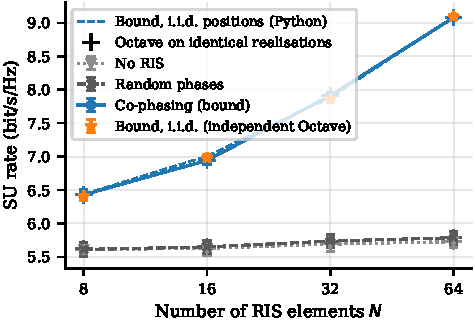
\includegraphics[width=\columnwidth]{fig1_rate_vs_N}
\caption{SU rate vs.\ $N$ without the PU constraint ($P=\Pmax$). Octave recomputation on identical realisations (+) and an independent Octave generator ($\star$) overlay the Python curves.}\label{fig:n}\end{figure}

\subsection{Optimisation baselines}
Without the constraint, co-phasing grows from \CFeight\ to \CFsixtyfour\,bit/s/Hz between $N=8$ and $64$, while random phases stay at the no-RIS level (Fig.~\ref{fig:n}). Under the constraint (Figs.~\ref{fig:pmax}--\ref{fig:ith}), all methods saturate once $\Pmax$ exceeds the interference-limited power. Above that point, the gap between PU-agnostic co-phasing and the PU-aware methods is what the RIS buys by steering energy away from the PU. The element-wise heuristic nearly closes this gap, and the joint SDR meets its own upper bound.

\begin{figure}[t]\centering\includegraphics[width=\columnwidth]{fig2_rate_vs_Pmax}
\caption{SU rate vs.\ $\Pmax$ ($N=16$, $\Ith=-90$\,dBm). Error bars: 95\% CI.}\label{fig:pmax}\end{figure}
\begin{figure}[t]\centering\includegraphics[width=\columnwidth]{fig3_rate_vs_Ith}
\caption{SU rate vs.\ $\Ith$ ($N=16$, $\Pmax=20$\,dBm).}\label{fig:ith}\end{figure}

\subsection{Learning}
%TD3-RESULTS%

\begin{figure*}[t]\centering\includegraphics[width=\textwidth]{fig4_learning_curves}
\caption{Validation rate during training (mean $\pm$ std over seeds). (a) Main agents vs.\ baseline levels. (b) Ablations at equal step counts.}\label{fig:lc}\end{figure*}

\input{table2}

\begin{figure}[t]\centering\includegraphics[width=\columnwidth]{fig6_runtime_vs_N}
\caption{Time per decision vs.\ $N$ (single thread, log scale). The TD3 time is architecture-bound and does not depend on the weights.}\label{fig:rt}\end{figure}
\begin{figure}[t]\centering\includegraphics[width=\columnwidth]{fig5_rate_along_trajectory}
\caption{SU rate along test flight 0 (1.6\,s, 200 decisions).}\label{fig:traj}\end{figure}

\subsection{Integrated sensing and communication}
MUSIC attains $\sqrt{\mathrm{CRB}}$ above its SNR threshold and then reaches the grid floor (Fig.~\ref{fig:music}). With fewer snapshots than antennas, MUSIC does not break down for a single target. Only its threshold moves, because only the principal eigenvector is needed. In the trade-off (Fig.~\ref{fig:isac}), the 8-antenna UAV nulls the PU for data, reaching $R=\RateISAC$\,bit/s/Hz. Isotropic probing, however, remains interference-limited, with a median echo SNR of \EchoIso\,dB. Restricting probes to the PU null space raises it to \EchoNull\,dB. At $\rho=0.1$ this cuts the median localisation error from \LocIsoTen\ to \LocNullTen\,m, and the 5\,m outage from \OutIsoTen\% to \OutNullTen\%, which is comparable to doubling the frame length.

\begin{figure}[t]\centering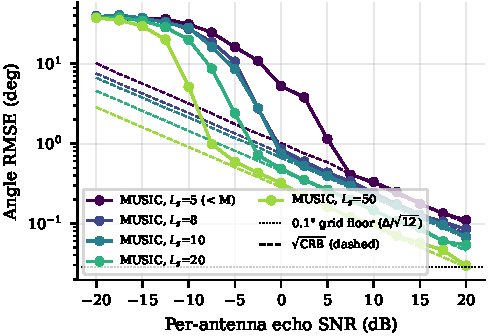
\includegraphics[width=\columnwidth]{fig7_music_rmse_vs_snr}
\caption{Angle RMSE of MUSIC (markers) and $\sqrt{\mathrm{CRB}}$ (dashed) vs.\ per-antenna echo SNR, $M=8$, 500 trials per point.}\label{fig:music}\end{figure}
\begin{figure}[t]\centering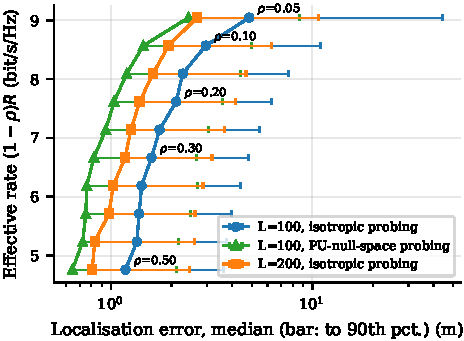
\includegraphics[width=\columnwidth]{fig8_isac_tradeoff}
\caption{Effective rate vs.\ localisation error as the sensing fraction $\rho$ increases (500 trials, common random numbers across $\rho$).}\label{fig:isac}\end{figure}

\section{Discussion and Limitations}
Learning is only worth its training cost if it beats cheap model-based alternatives on the metric that matters. Here, strong structure (co-phasing, projection, a tight SDR) makes the element-wise heuristic a demanding baseline. The honest role of DRL is therefore that of a fixed-latency approximator whose cost does not grow with the number of sweeps or with solver iterations, and the residual design is what makes it competitive. Limitations: perfect current CSI of the PU cascade is assumed (one-step-old CSI results are reported in Table~\ref{tab:main}); RIS elements are isotropic with no wall shadowing; and position error assumes a known range.

\section{Conclusion}
We showed that (P1) is an exact rank-constrained SDP whose relaxation was tight on every test state, identified why alternating power updates stall, and showed that DRL for RIS control needs a periodic action representation and physics-informed structure to be competitive at a fixed latency. For ISAC, PU-aware probing is the lever that matters under interference limits.

\begin{thebibliography}{9}\footnotesize
\bibitem{wu2019} Q.~Wu and R.~Zhang, ``Intelligent reflecting surface enhanced wireless network via joint active and passive beamforming,'' \emph{IEEE Trans. Wireless Commun.}, 2019.
\bibitem{huang2020} C.~Huang, R.~Mo, and C.~Yuen, ``Reconfigurable intelligent surface assisted multiuser MISO systems exploiting deep reinforcement learning,'' \emph{IEEE J. Sel. Areas Commun.}, 2020.
\bibitem{fujimoto2018} S.~Fujimoto, H.~van~Hoof, and D.~Meger, ``Addressing function approximation error in actor-critic methods,'' in \emph{Proc. ICML}, 2018.
\bibitem{raffin2021} A.~Raffin \emph{et al.}, ``Stable-Baselines3: Reliable reinforcement learning implementations,'' \emph{J. Mach. Learn. Res.}, 2021.
\bibitem{luo2010} Z.-Q.~Luo \emph{et al.}, ``Semidefinite relaxation of quadratic optimization problems,'' \emph{IEEE Signal Process. Mag.}, 2010.
\bibitem{zeng2016} Y.~Zeng, R.~Zhang, and T.~J.~Lim, ``Wireless communications with unmanned aerial vehicles: Opportunities and challenges,'' \emph{IEEE Commun. Mag.}, 2016.
\bibitem{liu2022} F.~Liu \emph{et al.}, ``Integrated sensing and communications: Toward dual-functional wireless networks for 6G and beyond,'' \emph{IEEE J. Sel. Areas Commun.}, 2022.
\bibitem{schmidt1986} R.~Schmidt, ``Multiple emitter location and signal parameter estimation,'' \emph{IEEE Trans. Antennas Propag.}, 1986.
\bibitem{stoica1989} P.~Stoica and A.~Nehorai, ``MUSIC, maximum likelihood, and Cram\'er--Rao bound,'' \emph{IEEE Trans. Acoust., Speech, Signal Process.}, 1989.
\bibitem{boyd2004} S.~Boyd and L.~Vandenberghe, \emph{Convex Optimization}. Cambridge Univ. Press, 2004.
\end{thebibliography}
\end{document}
